\documentclass[a4paper,11pt]{article}

% ------------------------------------------------------------
% Packages
% ------------------------------------------------------------
\usepackage[utf8]{inputenc}
\usepackage[T1]{fontenc}
\usepackage{lmodern}
\usepackage{amsmath,amssymb,amsthm}
\usepackage{geometry}
\usepackage{graphicx}
\usepackage{booktabs}
\usepackage{array}
\usepackage{enumitem}
\usepackage{microtype}
\usepackage{xcolor}
\usepackage{hyperref}
\usepackage{float}
\usepackage{caption}
\usepackage{subcaption}
\usepackage{algorithm}
\usepackage{algpseudocode}

\geometry{
    a4paper,
    left=1.8cm,
    right=1.8cm,
    top=1.5cm,
    bottom=1.5cm
}

\setlength{\parindent}{0pt}
\setlength{\parskip}{0.55em}

\hypersetup{
    colorlinks=true,
    linkcolor=black,
    citecolor=black,
    urlcolor=blue
}

% ------------------------------------------------------------
% Helper commands
% ------------------------------------------------------------
\newcommand{\norm}[1]{\left\lVert #1 \right\rVert}
\newcommand{\R}{\mathbb{R}}
\newcommand{\TODO}[1]{\textcolor{red}{\textbf{[TODO: #1]}}}

% ------------------------------------------------------------
% Document information
% ------------------------------------------------------------
\title{\textbf{Mixed-Precision Gram--Schmidt Orthogonalisation}\\[0.4em]
\large Software Practical Report}
\author{Lucia Hirsch}
\date{\today}

\begin{document}

\maketitle

% ============================================================
\section{Introduction and Motivation}
% ============================================================

Floating-point arithmetic is fundamental to numerical computing. It provides a
practical approximation to real-number arithmetic while allowing arithmetic
operations to be implemented efficiently on digital hardware. The IEEE
floating-point standards established a common framework for representing and
manipulating floating-point numbers and have consequently played an important
role in the reproducibility and portability of numerical software.

Traditionally, numerical algorithms have often been implemented using one
fixed floating-point precision throughout the complete computation. Double
precision, for example, is a common default when numerical stability is
important. This approach is simple and robust, but it is not necessarily
optimal. Not every operation in an algorithm contributes equally to the final
error, and not every intermediate quantity requires the same numerical
accuracy.

This motivates \emph{mixed-precision computing}: different parts of an
algorithm are evaluated using different floating-point formats. The central
idea is to spend high precision where it matters and use lower precision where
the resulting error is acceptable. In modern computing this is particularly
relevant because low-precision arithmetic is increasingly used in machine
learning and other large-scale workloads. Reduced precision can lower storage
requirements and, when supported directly by hardware, can also reduce
execution time and energy consumption.

The present practical investigates this idea for the
Gram--Schmidt orthogonalisation process. The main questions are:

\begin{enumerate}[label=(\roman*)]
    \item How does reducing the precision affect the numerical accuracy of
    Gram--Schmidt orthogonalisation?
    \item Do different operations of the algorithm have different precision
    requirements?
    \item Can increasing the precision of only selected operations improve
    stability?
    \item Can reorthogonalisation benefit from using a lower precision in the
    first pass and a higher precision in the second pass?
\end{enumerate}

The project therefore does not treat ``precision'' as a single parameter.
Instead, the implementation makes it possible to assign precisions to several
distinct stages of the algorithm.

An important limitation has to be stated at the outset. The experiments use
software libraries to emulate floating-point formats that are not necessarily
available as native arithmetic on the experimental machine. Consequently, the
present work evaluates numerical accuracy rather than actual speed, energy
consumption, or hardware-level savings. The implementation uses HDNUM, CPFloat
and GMP for the available precision formats.

% ============================================================
\section{Background}
% ============================================================

\subsection{Floating-point precision and unit roundoff}

A floating-point format can be characterised by, among other parameters, its
significand precision and exponent range. Rounding after an arithmetic
operation introduces a relative error whose typical scale is described by the
unit roundoff $u$. For a binary floating-point format with $p$ significant
bits, the unit roundoff is commonly written as $u = 2^{-p}$ 
under the convention used in this practical.

The different formats considered in the project have substantially different
precision and exponent ranges. In particular, formats with the same total
number of bits need not have the same numerical behaviour: allocating more
bits to the exponent increases the representable range, while allocating more
bits to the significand increases the precision of representable values.

\begin{table}[ht]
    \centering
    \caption{Floating-point formats considered in the experiments.
    The significand precision for normal numbers includes the implicit
    leading bit. $u$ denotes the unit roundoff, $x_{\min}$ the smallest
    positive normal value, $x_{\min,\mathrm{sub}}$ the smallest positive
    subnormal value, and $x_{\max}$ the largest finite value.}
    \label{tab:precisions}
    \begin{tabular}{lccccc}
        \toprule
        Format & (sig, exp) & $u$ & $x_{\min}$ & $x_{\min,\mathrm{sub}}$ & $x_{\max}$ \\
        \midrule
        FP8       & (4, 4)    & $6.25 \times 10^{-2}$
                  & $1.56 \times 10^{-2}$ & $1.95 \times 10^{-3}$
                  & $2.40 \times 10^{2}$ \\

        bfloat16  & (8, 8)    & $3.91 \times 10^{-3}$
                  & $1.18 \times 10^{-38}$ & $9.18 \times 10^{-41}$
                  & $3.39 \times 10^{38}$ \\

        FP16      & (11, 5)   & $4.88 \times 10^{-4}$
                  & $6.10 \times 10^{-5}$ & $5.96 \times 10^{-8}$
                  & $6.55 \times 10^{4}$ \\

        FP32      & (24, 8)   & $5.96 \times 10^{-8}$
                  & $1.18 \times 10^{-38}$ & $1.40 \times 10^{-45}$
                  & $3.40 \times 10^{38}$ \\

        FP64      & (53, 11)  & $1.11 \times 10^{-16}$
                  & $2.23 \times 10^{-308}$ & $4.94 \times 10^{-324}$
                  & $1.80 \times 10^{308}$ \\

        FP128     & (64, 64)  & $5.42 \times 10^{-20}$
                  & $2^{\,2-2^{63}}$
                  & $2^{\,3-2^{63}-64}$
                  & $(2-2^{-64})2^{2^{63}-1}$ \\

        FP256     & (192, 64) & $1.60 \times 10^{-58}$
                  & $2^{\,2-2^{63}}$
                  & $2^{\,3-2^{63}-192}$
                  & $(2-2^{-192})2^{2^{63}-1}$ \\

        FP512     & (448, 64) & $1.27 \times 10^{-135}$
                  & $2^{\,2-2^{63}}$
                  & $2^{\,3-2^{63}-448}$
                  & $(2-2^{-448})2^{2^{63}-1}$ \\

        FP1024    & (960, 64) & $1.87 \times 10^{-289}$
                  & $2^{\,2-2^{63}}$
                  & $2^{\,3-2^{63}-960}$
                  & $(2-2^{-960})2^{2^{63}-1}$ \\
        \bottomrule
    \end{tabular}
    \smallskip
    \parbox{0.95\textwidth}{\footnotesize
    For FP128--FP1024, the range values are given according to the assumed
    exponent convention and should be interpreted as theoretical values.
    The subnormal values are obtained by extending the normal range with
    the corresponding subnormal spacing.}
\end{table}

The distinction between precision and exponent range becomes particularly
important for the low-precision experiments. FP16 and bfloat16 both use
16 bits, but bfloat16 allocates more bits to the exponent. The experiments
show that this difference has practical consequences for Gram--Schmidt:
FP16 can encounter divisions by zero at substantially smaller condition
numbers, whereas bfloat16 does not exhibit the same failure in the tested
range.

\subsection{Gram--Schmidt orthogonalisation}

Given a matrix $A= [a_1,...,a_n] \in\R^{m\times n}$,
Gram--Schmidt constructs an orthogonal matrix $Q=[q_1,...,q_n]$
to an upper triangular matrix $R$ such that
\[
    A \approx QR.
\]
In exact arithmetic, the columns of $Q$ are orthonormal:
\[
    Q^TQ=I.
\]

The basic Gram--Schmidt step consists of computing projections of a column
onto previously computed orthogonal vectors, subtracting those projections,
and finally normalising the resulting vector.

For classical Gram--Schmidt (CGS), all projections of a vector are computed
against the previously constructed vectors before the vector is updated. In
modified Gram--Schmidt (MGS), the update is performed after each projection.
This difference changes the numerical behaviour of the two algorithms.

A second application of Gram--Schmidt is commonly used for
\emph{reorthogonalisation}. The resulting CGS2 and MGS2 variants perform the
orthogonalisation twice. Reorthogonalisation can substantially improve the
orthogonality of the computed basis, although the additional computation also
creates further opportunities for rounding errors.

% ============================================================
\section{Mixed-Precision Variant}
% ============================================================

\subsection{Design of the implementation}

The implementation extends the conventional Gram--Schmidt algorithms so that
up to four different precision types can be selected independently. They are
denoted by $T_1,\ldots,T_4$:

\begin{description}[leftmargin=2.8cm,style=nextline]
    \item[$T_1$ -- storage precision]
    The input and output matrix entries are stored in this precision. Results
    of intermediate operations are eventually cast back to $T_1$ when they
    are stored.

    \item[$T_2$ -- inner-product precision]
    Dot products and the corresponding accumulated sums are evaluated in this
    precision. Since inner products repeatedly accumulate rounding errors,
    this operation was expected to have a particularly strong influence on
    numerical accuracy.

    \item[$T_3$ -- projection/AXPY precision]
    Projection updates and AXPY-type operations are evaluated after casting
    their operands to $T_3$. The resulting entries are subsequently converted
    back to $T_1$.

    \item[$T_4$ -- normalisation precision]
    The normalisation stage is evaluated in this precision. The vector entries
    are converted to $T_4$, the required norm is computed, the division is
    performed, and the result is cast back to $T_1$.
\end{description}

This separation is useful experimentally because it makes it possible to
isolate the effect of a particular operation. Instead of merely asking whether
``FP32 is better than FP16'', one can ask, for example, whether keeping the
inner product in FP64 while performing the remaining operations in FP32 is
beneficial.

\subsection{Casting between precisions}

The implementation requires conversions between the supported numerical types.
The conversion mechanism uses the existing constructors of the relevant
classes. In particular, CPFloat and GMP values can be converted through their
stored double representation where necessary.

The practical therefore does not introduce a new floating-point arithmetic
implementation. Instead, it provides an interface that allows the existing
algorithmic operations to be performed on values represented by different
precision types.

\subsection{Classical and modified Gram--Schmidt}

The classical Gram--Schmidt implementation follows the existing HDNUM
implementation, with the important modification that the individual
operations call the precision-conversion functionality.

The inner-product stage stores the accumulated sum in $T_2$ and casts the
vector entries to $T_2$ before multiplication and addition. The projection
stage casts the relevant values to $T_3$, performs the AXPY-like update, and
stores the result back in $T_1$. Finally, normalisation uses the selected
normalisation precision.

MGS is implemented analogously, with the difference being the order in which
columns are updated, as required by modified Gram--Schmidt.

\subsection{Reorthogonalisation}

For CGS2 and MGS2, the implementation uses two different experimental
configurations.

With four template parameters, the same four precision choices are used for
both orthogonalisation passes. This permits mixed precision between operation
types while keeping the implementation interface unchanged.

A second configuration uses two precision parameters to investigate a
different question: whether a lower-precision first orthogonalisation followed
by a higher-precision reorthogonalisation can compete with simply performing
the complete computation in the higher precision. In this implementation,
CGS/MGS is first executed uniformly in the lower precision. The result is
then cast to the higher precision and CGS/MGS is executed again uniformly in
that higher precision.
The results of this configuration are compared with a uniform high-precision
baseline.

% ------------------------------------------------------------
\subsection{Pseudocode}
% ------------------------------------------------------------

The following pseudocode abstracts the implementation and emphasises where
the four precision parameters enter. The exact C++ function names are omitted
so that the algorithmic structure is independent of the implementation
details.

\begin{algorithm}[H]
\caption{Mixed-Precision Classical Gram--Schmidt}
\label{alg:cgs-mixed}
\begin{algorithmic}[1]
\Require $A\in\mathbb{R}^{m\times n}$ and precisions $T_1,T_2,T_3,T_4$
\State $Q\gets A$ \Comment{stored in $T_1$}
\For{each column $k$ except first}
    \For{each previous column $j$}
        \State Compute $q_j^Ta_k$ and $q_j^Tq_j$ in $T_2$,
        casting $a_k \in A, q_j \in Q$ to $T_2$
        \State $\alpha\gets
        \operatorname{cast}_{T_3}(q_j^Ta_k)/
        \operatorname{cast}_{T_3}(q_j^Tq_j)$
        \State Update $q_k\gets q_k-\alpha q_j$ in $T_3$,
        then cast the result to $T_1$
    \EndFor
\EndFor
\For{each column $q_j$}
    \State Compute $\norm{q_j}$ in $T_4$, casting $q_j \in Q$ to $T_4$
    \State Normalize $q_j$ in $T_4$ and cast the result to $T_1$
\EndFor
\State \Return $Q$
\end{algorithmic}
\end{algorithm}

For MGS, the same precision separation is used, but the vector is updated
after each projection. CGS2 and MGS2 apply the corresponding orthogonalisation
procedure twice.

% ============================================================
\section{Numerical Error Measures}
% ============================================================

Two error measures are used throughout the experiments.

\subsection{Loss of orthogonality}

Since the columns of an ideal orthogonal matrix satisfy
\[
    Q^TQ=I,
\]
the loss of orthogonality is measured by
\[
    E_{\mathrm{orth}}
    =
    \norm{Q^TQ-I}.
\]
This quantity directly measures how far the computed basis is from being
orthogonal.

\subsection{Representation error}

The second metric evaluates whether the computed factors still represent the
original matrix:
\[
    E_{\mathrm{rep}}
    =
    \frac{\norm{A-QR}}{\norm{A}}.
\]
This is a relative reconstruction error.

The distinction between the two metrics is important. A method can produce
vectors that are highly orthogonal while introducing a relatively large
representation error. This distinction becomes particularly visible in the
mixed-precision reorthogonalisation experiments.

% ============================================================
\section{Experimental Setup}
% ============================================================

The experimental framework was designed to compare different combinations of
algorithm and precision while varying the conditioning of the input problem.
The principal algorithms are CGS, MGS, CGS2 and MGS2.

\subsection{Precision configurations}

The experiments cover three broad classes of precision:

\begin{enumerate}
    \item low precision supplied by CPFloat, including FP8, FP16 and bfloat16;
    \item native single and double precision;
    \item high precision supplied through GMP, including FP128, FP256,
    FP512 and FP1024.
\end{enumerate}

The high-precision experiments are particularly useful for determining whether
an operation is limited by the precision of the arithmetic in that operation
or by the precision in which the data are ultimately stored.

\subsection{Conditioning}

The experiments vary the condition number of the input matrix from $10^{1}$ to $10^{16}$. This is
important because Gram--Schmidt becomes progressively more difficult as the
columns of the matrix become increasingly ill-conditioned. These input matrices $A \in\R^{100\times 10}$ were
generated using the provided header file. The seeds used are documented in the
file names of the graphs. For all experiments included in this report the same settings were used.

The expected behaviour for CGS/MGS is $\norm{Q^TQ-I} = O(\kappa (A) \cdot u)$, and $\norm{Q^TQ-I} = O(u)$
for CGS2/MGS2.

\subsection{Experimental categories}

The experiments can be divided into five categories:

\begin{enumerate}
    \item uniform-precision baselines;
    \item isolated higher precision for one operation type;
    \item high-precision inner products combined with low-precision
    projections and normalisation;
    \item mixed-precision reorthogonalisation;
    \item reduced precision for a single operation in an otherwise
    double-precision computation.
\end{enumerate}

This organisation separates two different questions. First, the baseline
experiments determine how the algorithms behave when the entire computation
uses one precision. Second, the mixed-precision experiments investigate
whether this behaviour can be improved by assigning precision selectively.

% ============================================================
\section{Results}
% ============================================================

\subsection{Uniform-precision baseline}

The first experiment establishes the behaviour of CGS, MGS, CGS2 and MGS2 when
all operations use the same precision. This is shown for all precisions excluding
GMP formats in Figure~\ref{fig:baseline-low}, as to retain a reasonable scale the y-axis.

For CGS and MGS, the expected qualitative behaviour is observed: as the
condition number increases, the error grows, reaching values of approximately
one for sufficiently difficult problems. Reorthogonalised variants are much
more stable over a substantial range of condition numbers.

An interesting observation is that FP16 appears more stable for CGS2 than for
MGS2 in parts of the tested range. The CGS2 error is also not perfectly
constant for very large condition numbers. Around a condition number of order
$\sqrt{1 / u}$ in the relevant scaling, both orthogonality and representation
errors begin to increase.

\begin{figure}[ht]
    \centering
    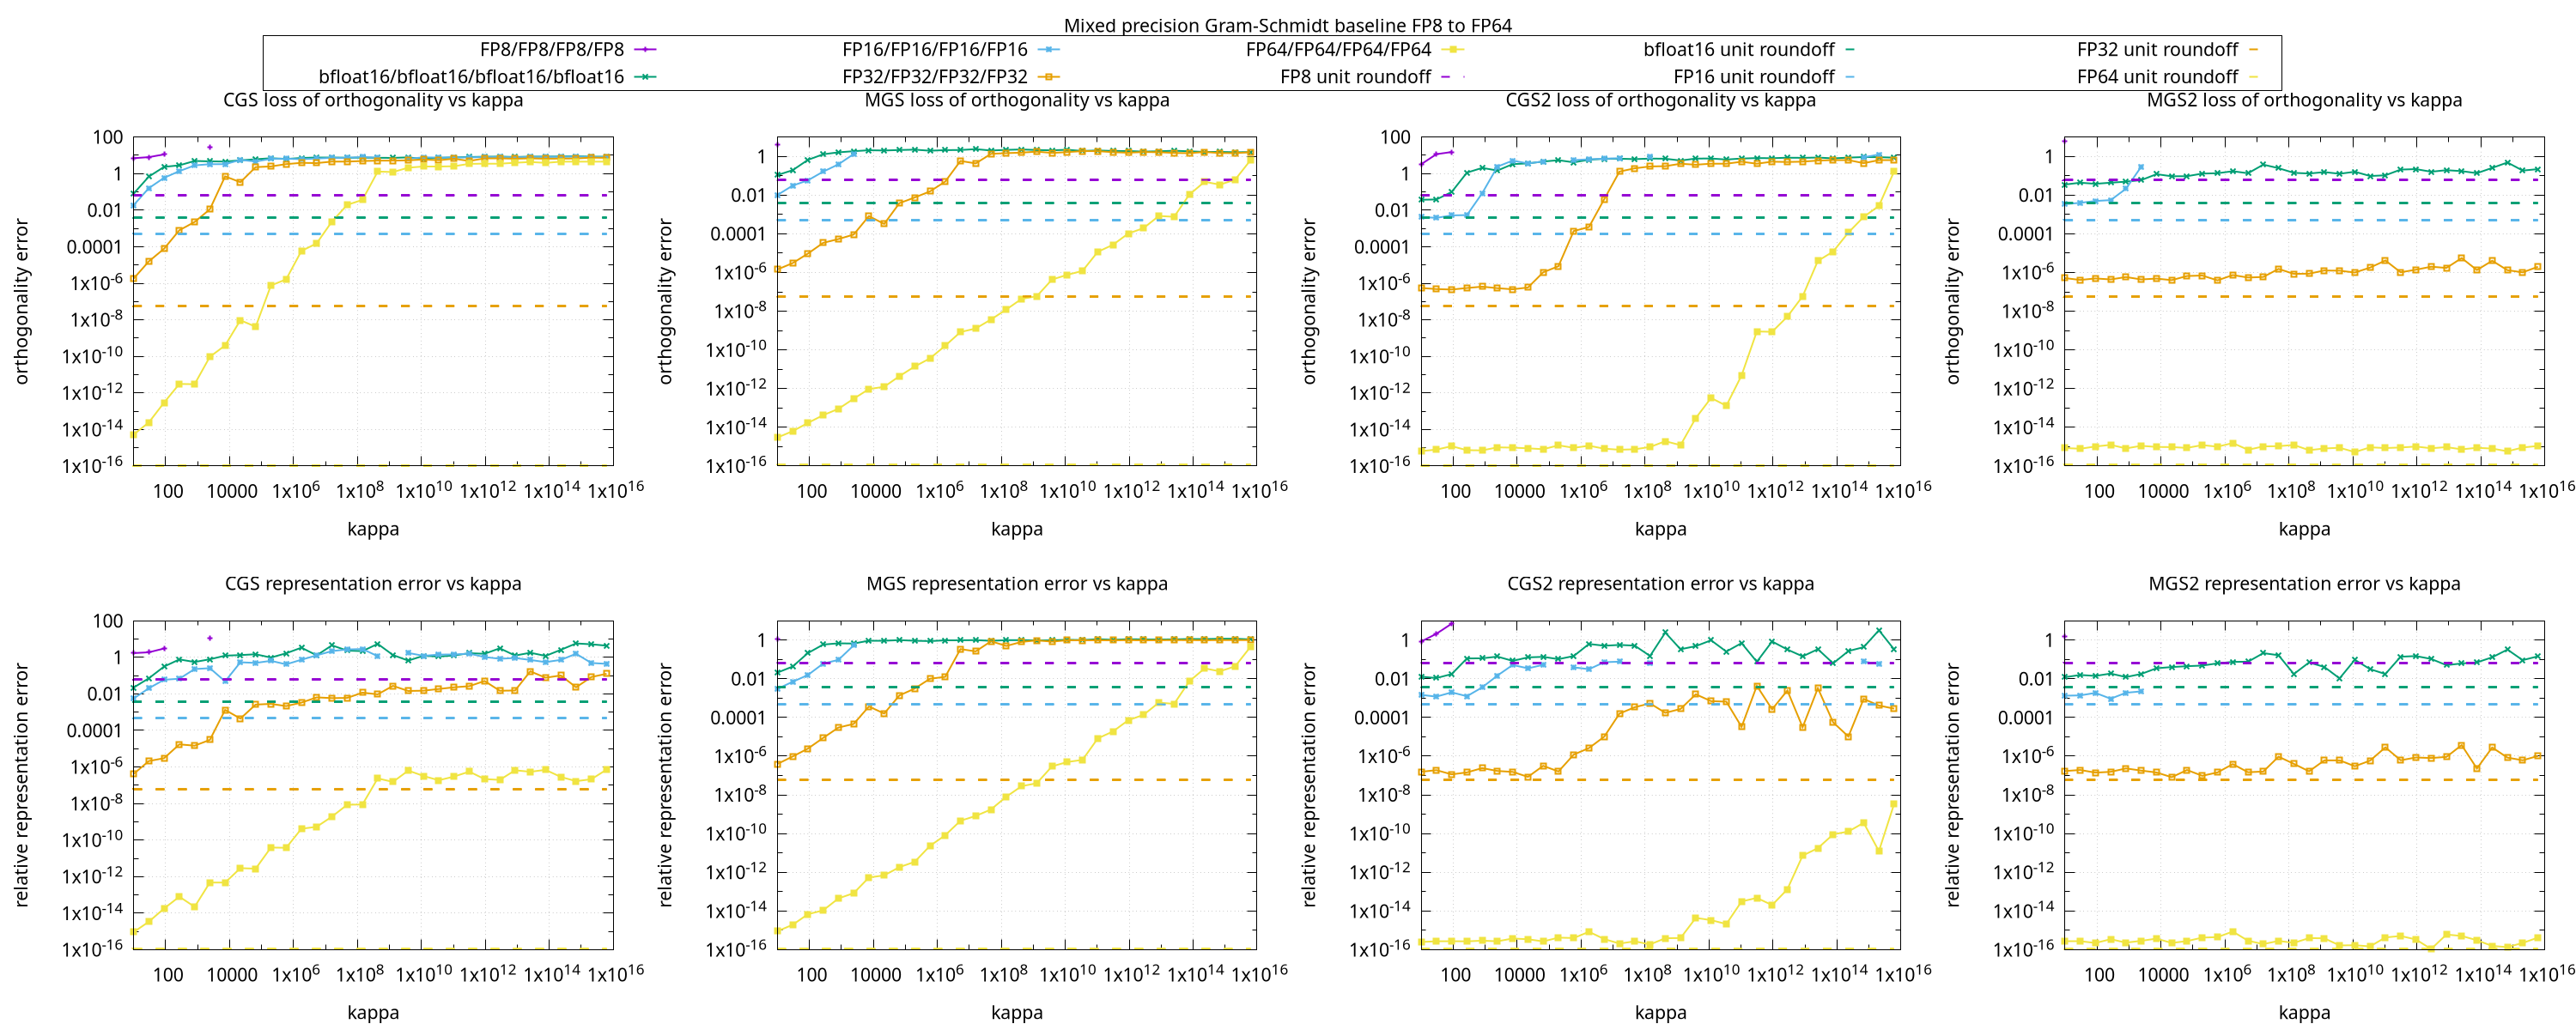
\includegraphics[width=\textwidth]{plots/mgs_plot_seed_u_v_730_169_2026-08-15_12-56.png}
    \caption{Uniform-precision baseline for low and native precisions.}
    \label{fig:baseline-low}
\end{figure}

\subsubsection{Failure of very low precision}

The low-precision experiments also reveal a practical limitation that is not
captured by the unit roundoff alone. FP8 and FP16 can fail because intermediate
values become too large or too small, leading to divisions by zero during
projection or normalisation. Table~\ref{tab:precision-cutoff} shows the
largest tested condition number for which each algorithm completed
successfully.

\begin{table}[ht]
    \centering
    \caption{Largest tested condition number for which the low-precision
    experiments completed successfully.}
    \label{tab:precision-cutoff}
    \begin{tabular}{lcc}
        \toprule
        Algorithm & FP8 & FP16 \\
        \midrule
        CGS  & $2.560\times10^2$ & $1.049\times10^6$ \\
        MGS  & $1.600\times10^1$ & $4.096\times10^3$ \\
        CGS2 & $3.200\times10^1$ & $8.192\times10^3$ \\
        MGS2 & $1.600\times10^1$ & $4.096\times10^3$ \\
        \bottomrule
    \end{tabular}
\end{table}

The bfloat16 format is the only low precision format that does not show the 
same failure in the tested range due to its
larger exponent range. The experiment therefore demonstrates that the total
number of bits is not sufficient to predict the behaviour of a low-precision
algorithm.

The FP16 result also suggests a possible direction for future work: scaling
the values closer to one before critical calculations and scaling them back
afterwards could potentially make FP16 more usable. This was not tested in
the present practical.

\subsection{High-precision baseline}

The second baseline considers the high-precision formats supplied through GMP.
Because the available precisions increase exponentially, a graph of all high-precision 
formats is not useful to observe the error behaviour and therefore not included here.

For low condition numbers, the errors are close to the unit roundoff and then
increase as expected with the condition number for CGS/MGS. For CGS2 and MGS2, the error initially
starts below the unit roundoff of the selected arithmetic but climbs linearly up to $u$ for 
increasing $\kappa(A)$, reflecting the effect of the reorthogonalisation procedure.

\subsection{Increasing the precision of one operation}

The next experiment isolates the effect of using a double precision for one
operation type while leaving the remaining operations at single
precision, as seen in Figure~\ref{fig:one-operation-native}.

For CGS and MGS without reorthogonalisation, higher-precision inner products
produce a modest improvement at low condition numbers, with an observed
reduction in error of roughly one order of magnitude. The other isolated
changes are much harder to distinguish from the baseline in the corresponding
plots.

For CGS2 and MGS2, the behaviour differs. At low condition numbers, higher
precision for normalisation appears to have the strongest effect. 
For this precision combination around
$\kappa(A)\approx10^7$, however, the relative behaviour changes: high-precision
inner products become the most effective isolated modification, improving the
error by approximately a factor of ten relative to the other variants.

\begin{figure}[ht]
    \centering
    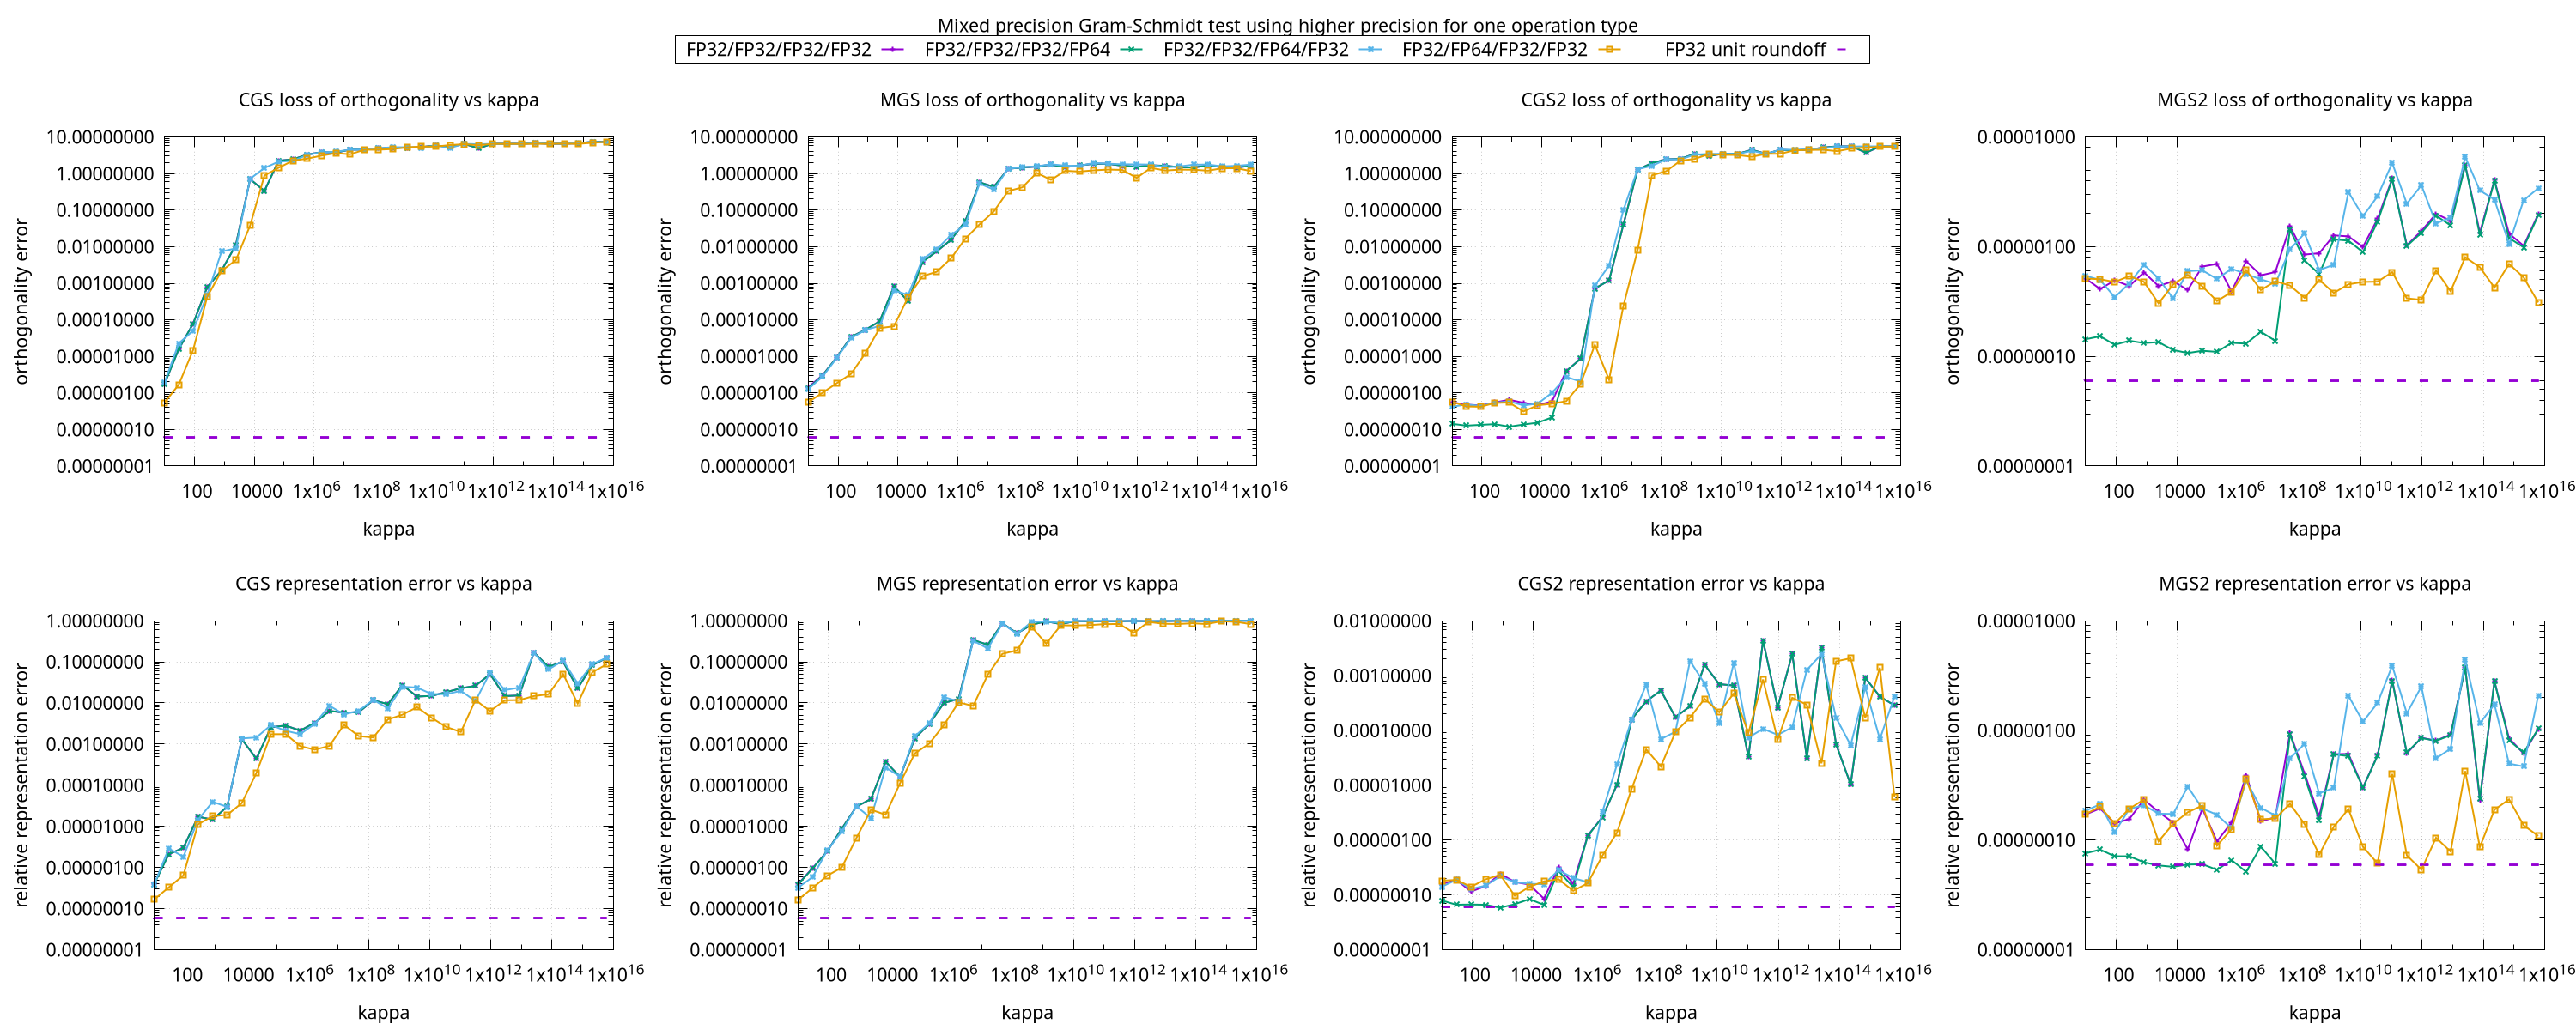
\includegraphics[width=\textwidth]{plots/mgs_plot_seed_u_v_730_169_2026-08-15_12-59.png}
    \caption{Using higher precision for a single operation type with native
    precision as the baseline.}
    \label{fig:one-operation-native}
\end{figure}

Repeating the experiment with double and GMP precisions produces the same qualitative
behaviour. The exact GMP precision makes little difference, 
Figure~\ref{fig:one-operation-gmp} shows FP128,
which is consistent with the fact that the data are still stored in double
precision. In that case, the storage precision $T_1$ can become the limiting
factor.

\begin{figure}[ht]
    \centering
    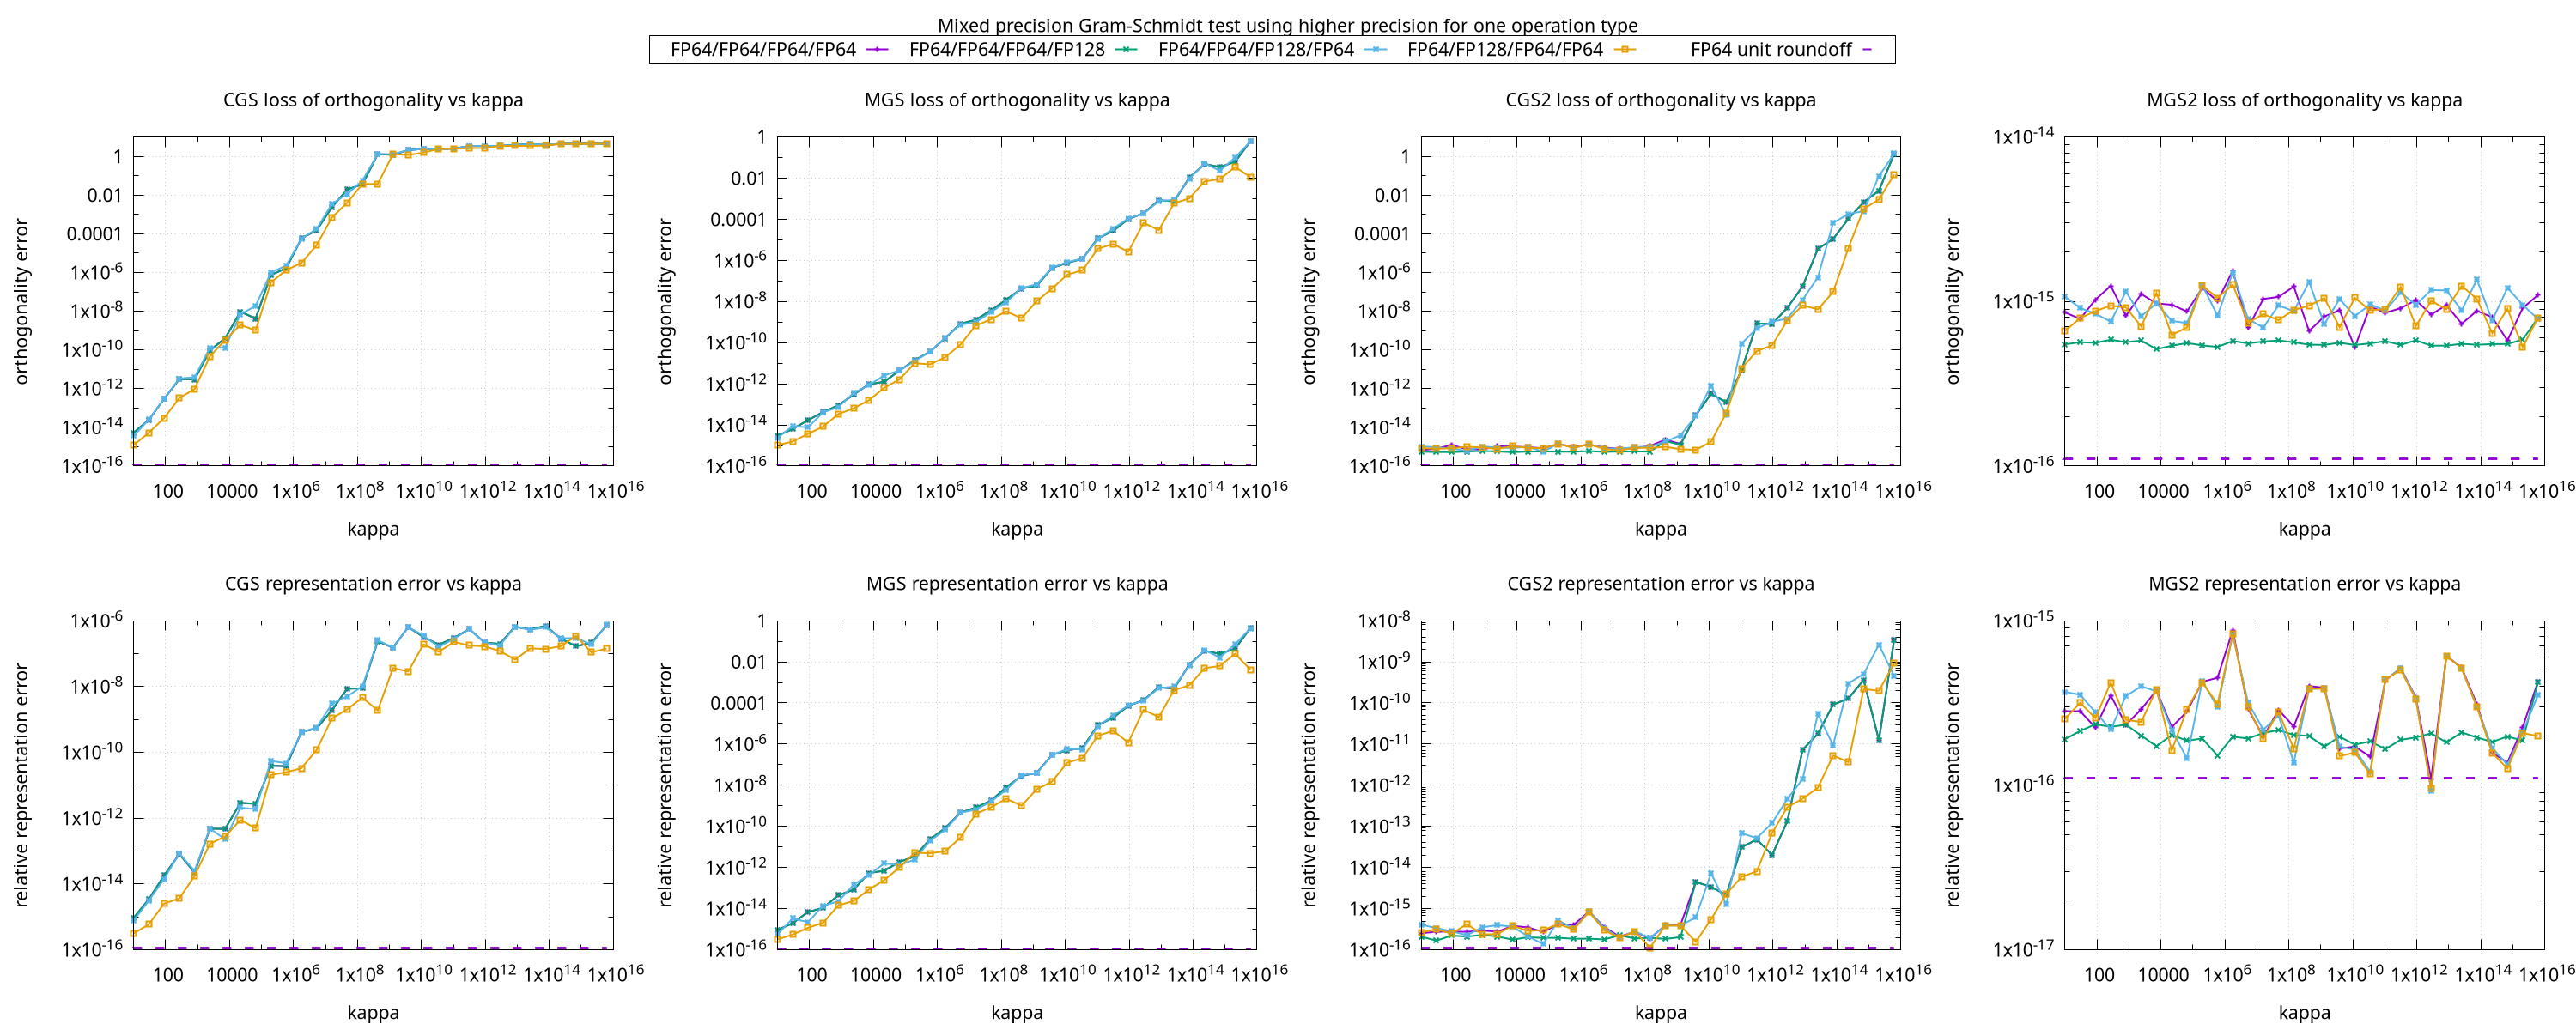
\includegraphics[width=\textwidth]{plots/mgs_plot_seed_u_v_730_169_2026-08-15_13-00.png}
    \caption{Using high GMP precision for one operation type.}
    \label{fig:one-operation-gmp}
\end{figure}

An exception is MGS2, where high-precision normalisation remains particularly
effective even at high condition numbers. This indicates that the numerical
importance of an operation depends not only on the operation itself but also
on the algorithmic variant in which it occurs.

\subsection{High-precision inner products with low-precision updates}

A more targeted experiment fixes projection and normalisation in a low
precision while performing inner products in a very high precision. This
tests whether accurate accumulation alone can compensate for the reduced
precision elsewhere.

The results seen in Figure~\ref{fig:high-dot-low-rest} are consistent with the preceding isolated-operation experiment,
but the improvements from the high-precision inner products are smaller than
might initially be expected. This indicates that accurate inner products are
not sufficient to recover the accuracy lost when subsequent projections and
normalisations are performed in low precision.

\begin{figure}[ht]
    \centering
    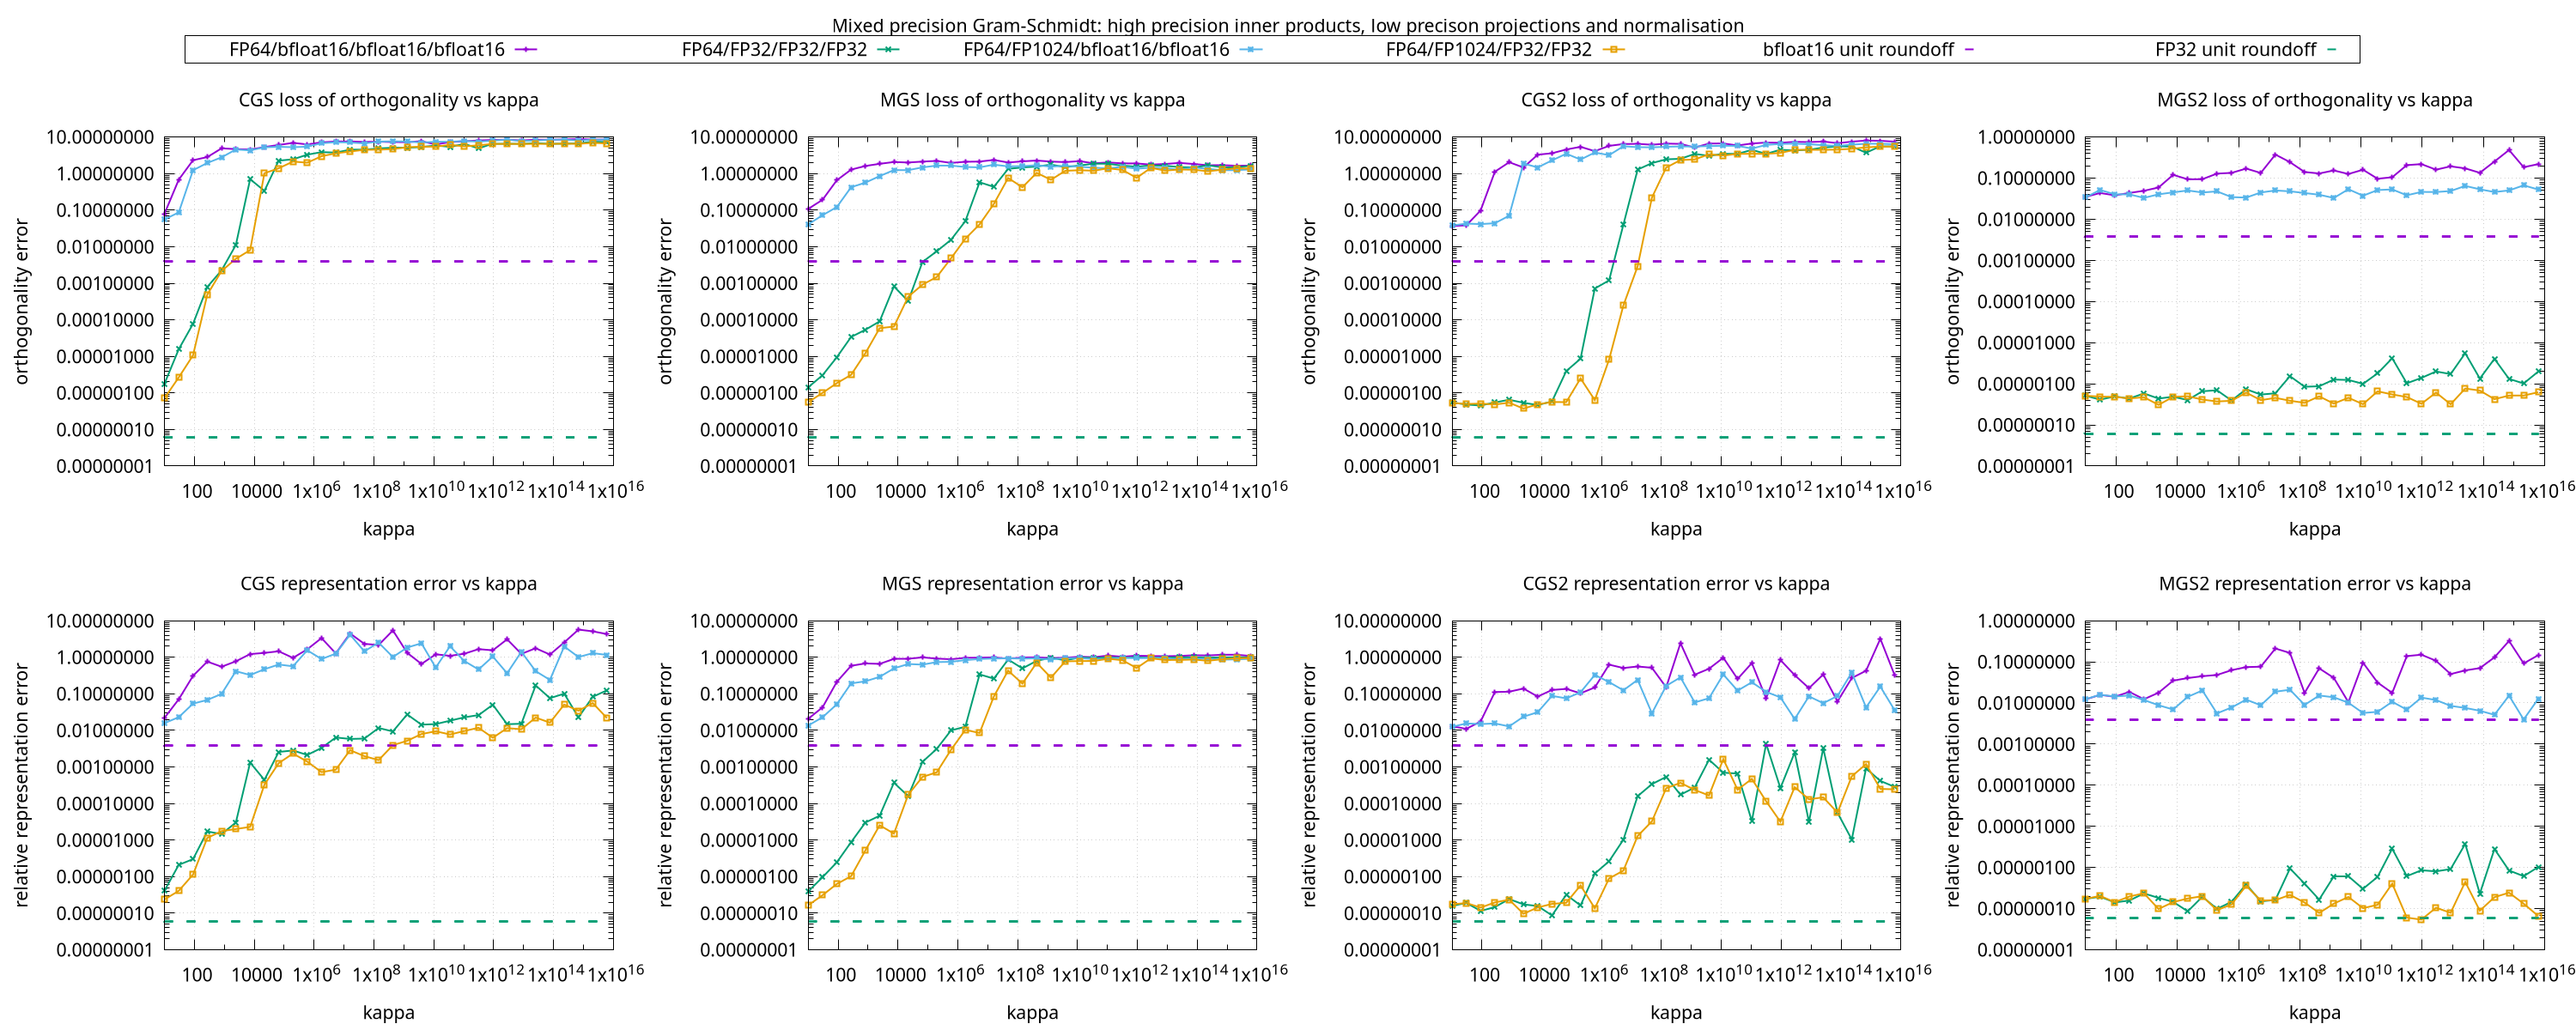
\includegraphics[width=\textwidth]{plots/mgs_plot_seed_u_v_730_169_2026-08-15_13-03.png}
    \caption{High-precision inner products combined with low-precision
    projection and normalisation.}
    \label{fig:high-dot-low-rest}
\end{figure}

This result illustrates an important principle of the mixed-precision
approach: increasing the precision of one operation cannot necessarily
overcome a later conversion to a lower-precision representation. If a
quantity is repeatedly rounded back to the storage precision, the benefit of
a more accurate intermediate calculation can be lost.

\subsection{Mixed-precision reorthogonalisation}

The next experiment investigates whether the first and second
orthogonalisation passes should use different precisions.

The key comparison is between a uniform high-precision computation and a
two-stage computation in which the first pass uses a lower precision and the
second pass uses a higher precision, see Figure~\ref{fig:mixed-reorth}. In particular, configurations using
bfloat16 or FP32 for the first pass and FP64 for the second pass were compared
with uniform FP64 and FP32 baselines.

The orthogonality results are striking. In CGS2, first performing the
orthogonalisation in bfloat16 can produce a surprisingly low and relatively
constant orthogonality error, in some regions even below the uniform FP32 and
FP64 variants.

However, this apparent improvement does not translate directly to the
representation error. The reconstruction error remains close to the unit
roundoff associated with the lower precision used in the first pass. Thus,
the two error measures tell a different story: the low-precision first pass results in a accuracy loss expected for that precision,
a second high-precision pass can recover orthogonality but not the representation of the original matrix.
However, this does not fully explain, why very low precisions produce better orthogonality
after reorthogonalisation.

\begin{figure}[ht]
    \centering
    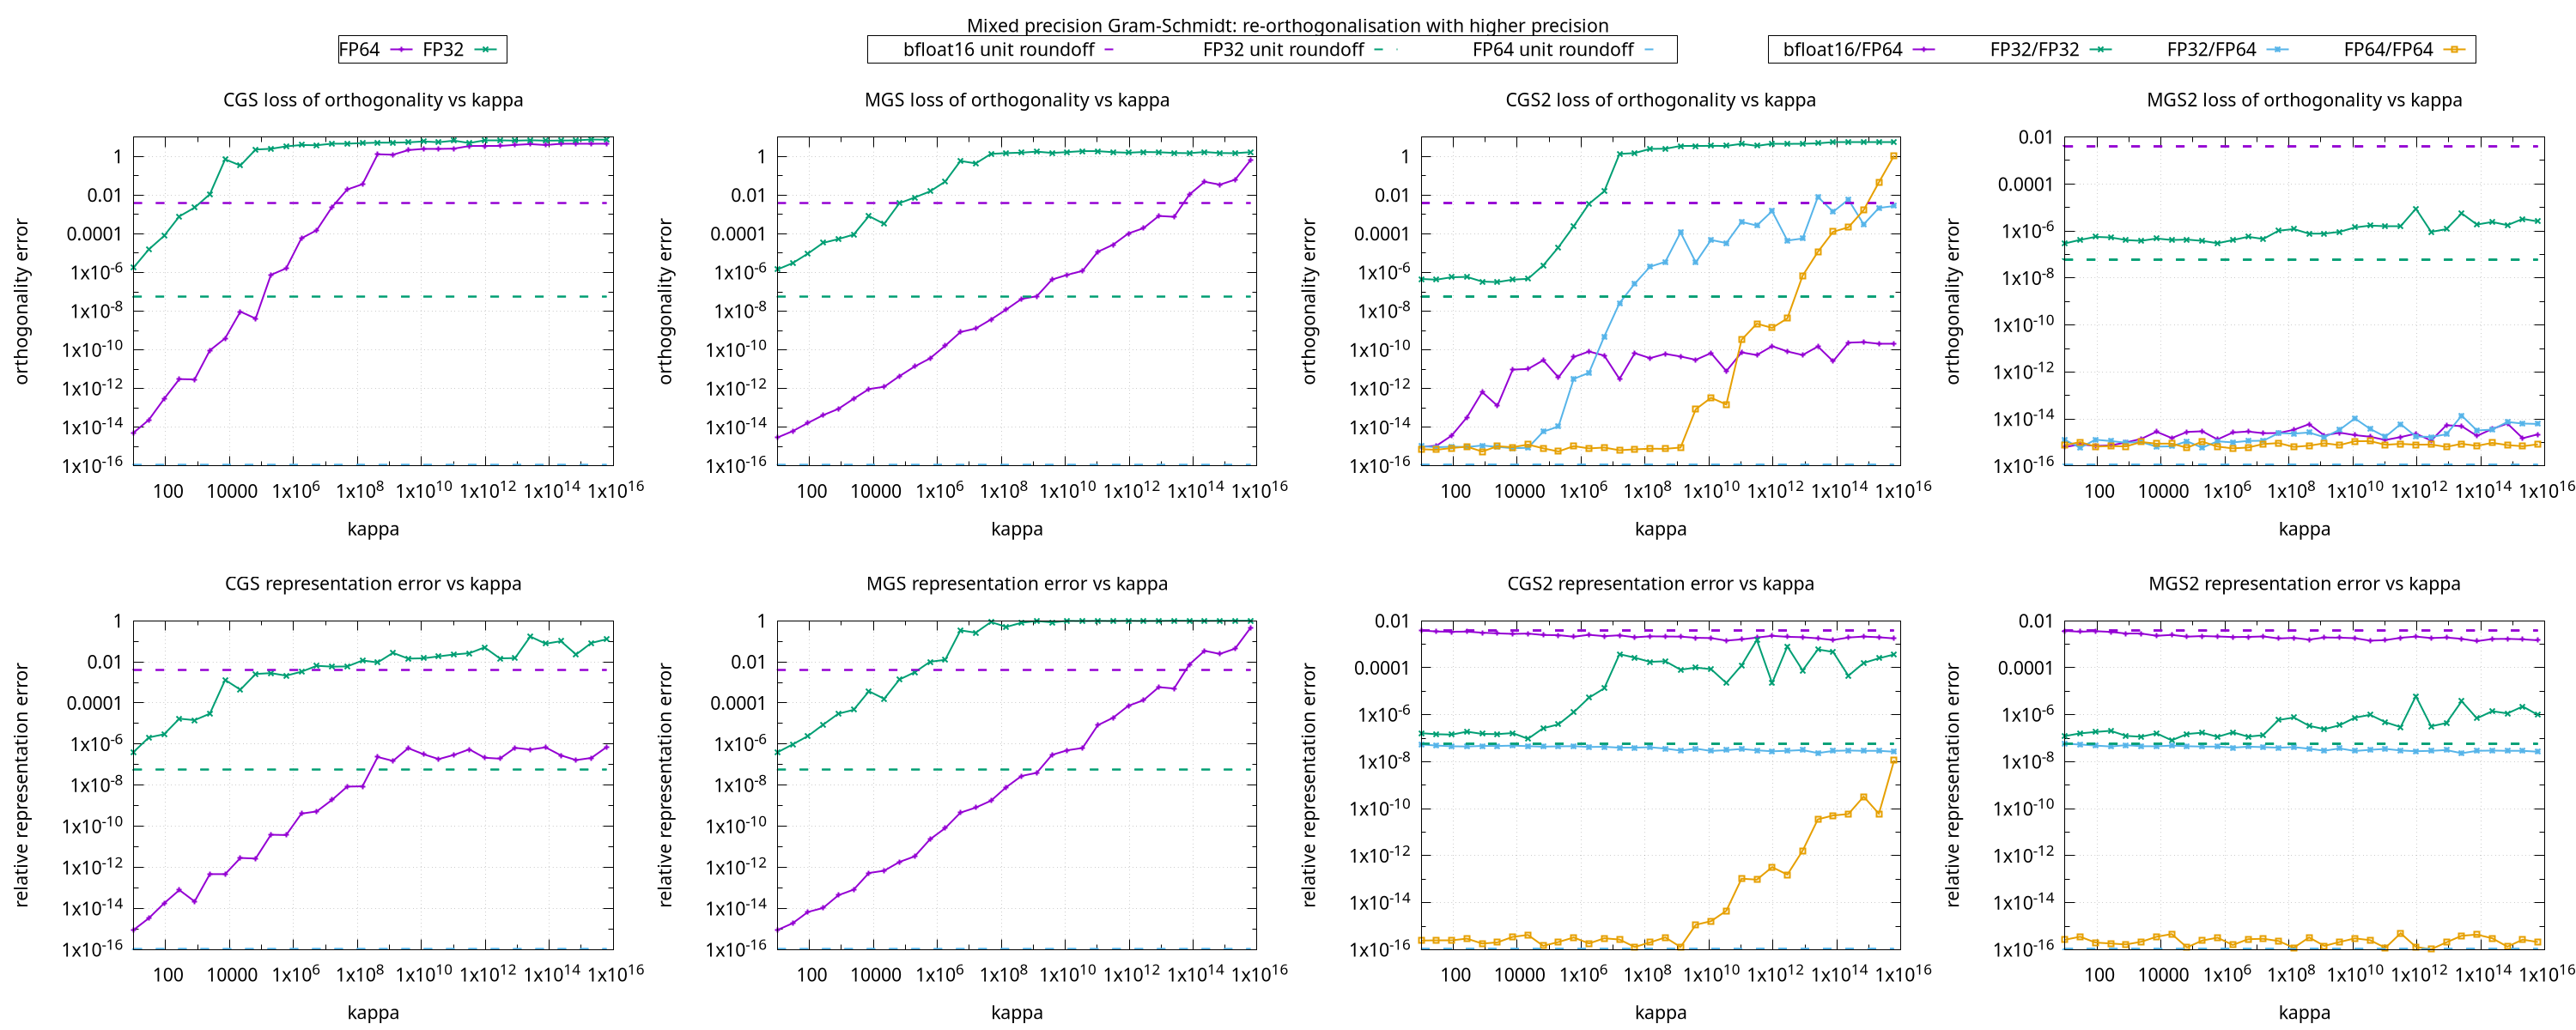
\includegraphics[width=\textwidth]{plots/mgs_plot_seed_u_v_730_169_2026-08-15_12-53.png}
    \caption{Low-precision first orthogonalisation and high-precision
    reorthogonalisation.}
    \label{fig:mixed-reorth}
\end{figure}

Among the tested configurations, FP32/FP64 appears particularly promising.
For high condition numbers it outperforms uniform FP64 CGS/MGS in both error
metrics in the reported experiments. Using still higher precisions did not
produce qualitatively new observations.

\subsection{Reducing the precision of one operation}

The final experiment approaches mixed precision from the opposite direction.
Instead of increasing the precision of one operation, the configuration shown in 
Figure~\ref{fig:saving-operation} starts from a
double-precision baseline and uses single precision for exactly one operation
type.

The expectation is that this configuration might identify operations whose
precision can be reduced at relatively little numerical cost. Unfortunately,
most variants perform almost as poorly as the uniform single-precision
baseline. The most notable exceptions involve the inner product and
normalisation stages.

Reducing the normalisation precision does not preserve the accuracy of the
double-precision baseline, but the resulting errors remain comparatively
constant around the single-precision unit roundoff. Reducing the projection
precision is slightly better than the uniform single-precision baseline in
one of the tested configurations.

A particularly unexpected result occurs for MGS2: using single precision
only for inner products produces substantially worse errors at high condition
numbers than using single precision for all operation types. The present
experiments do not provide a definitive explanation for this behaviour.

\begin{figure}[ht]
    \centering
    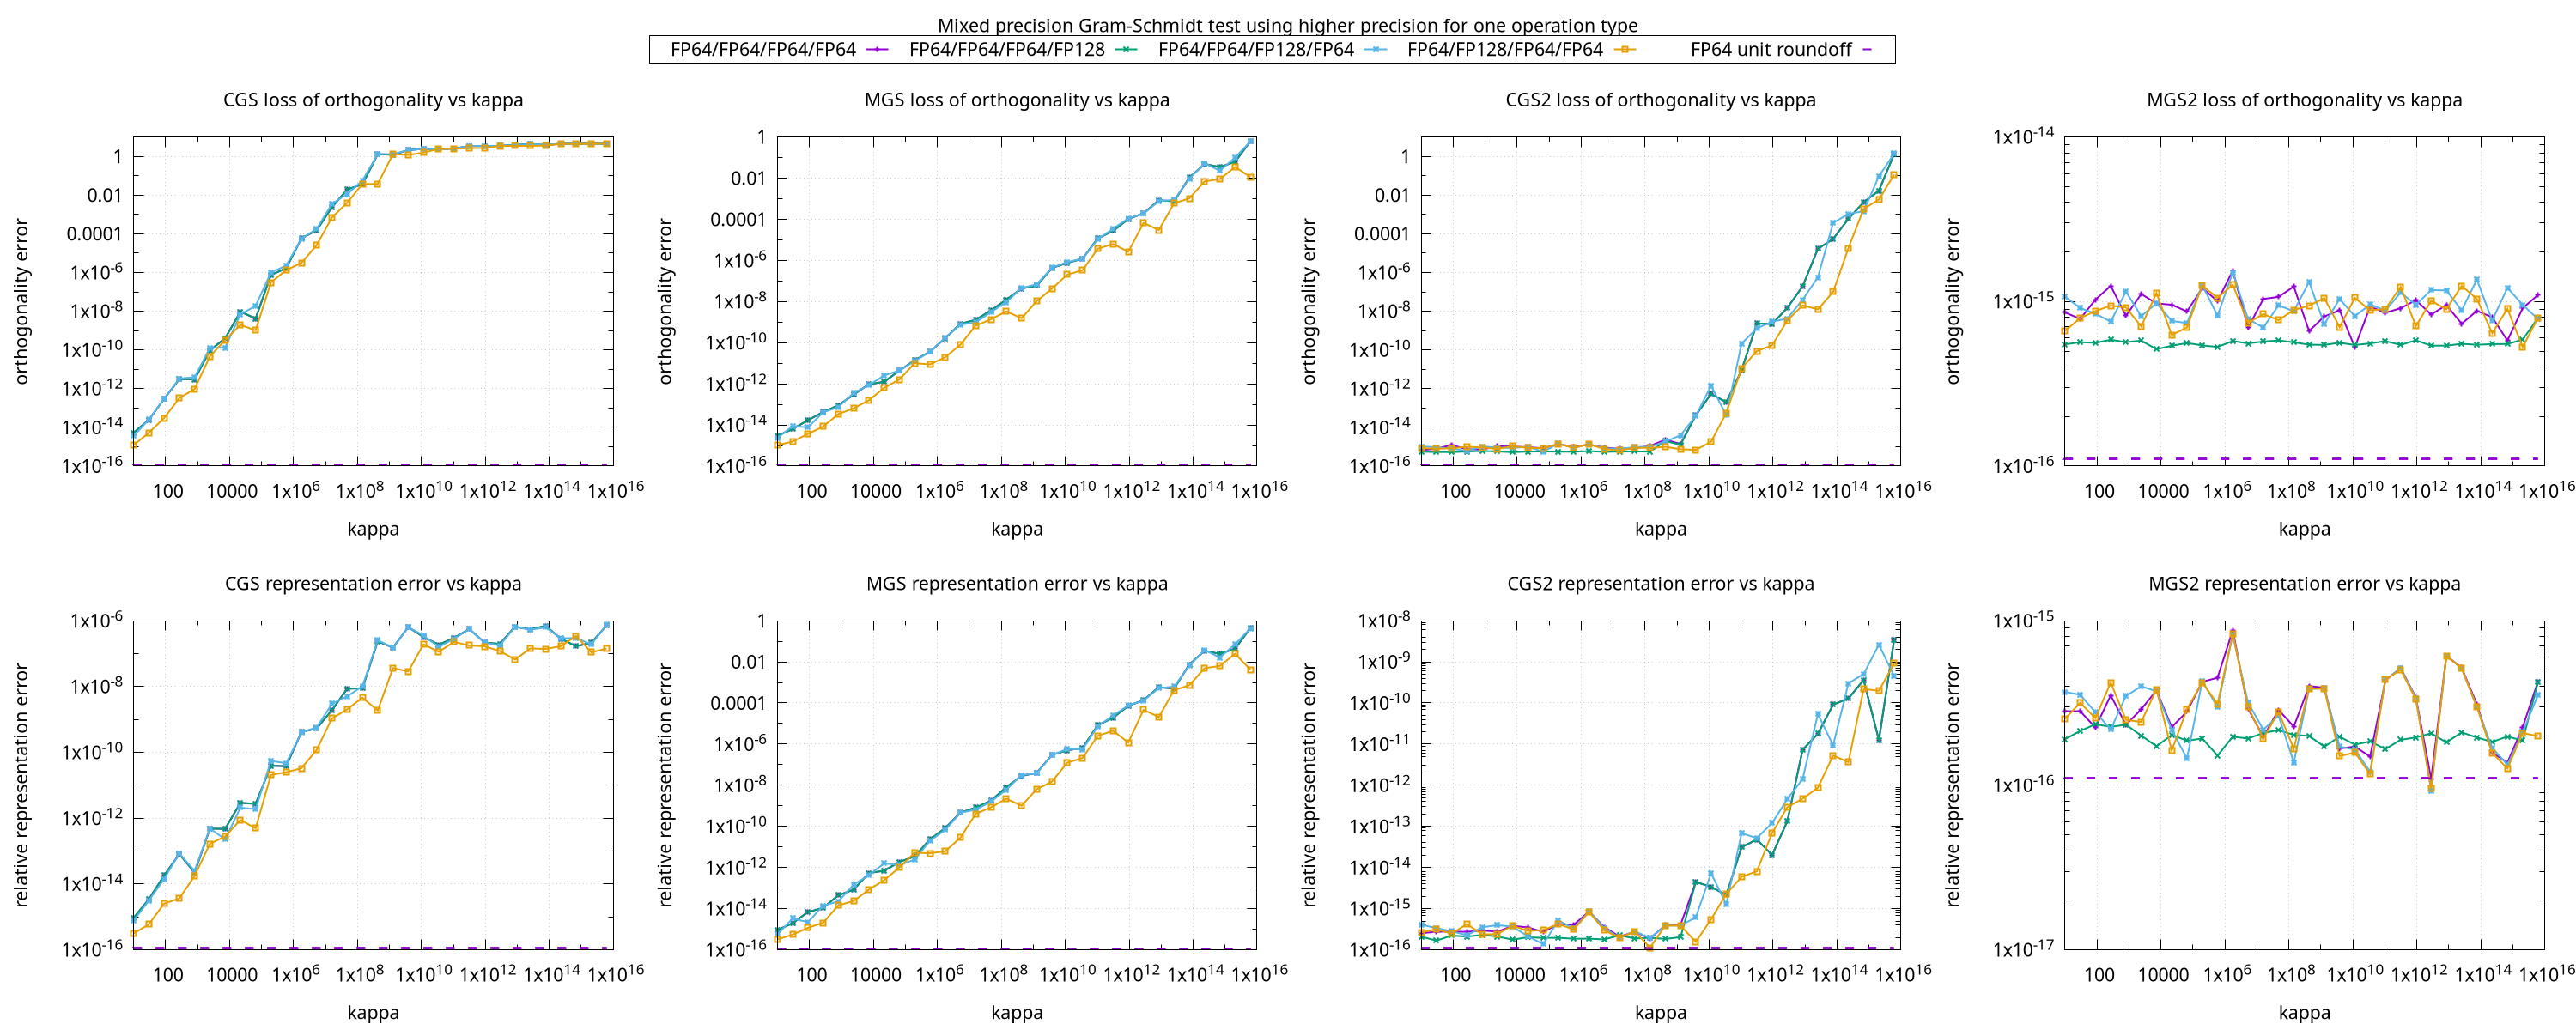
\includegraphics[width=\textwidth]{plots/mgs_plot_seed_u_v_730_169_2026-08-15_13-00.png}
    \caption{Reducing the precision of a single operation type. Replace this
    image with the final ``saving'' experiment plot if the filename differs
    from the draft.}
    \label{fig:saving-operation}
\end{figure}

Overall, this experiment is somewhat disappointing from the perspective of
``saving'' on recources but retaining comparable accuracy. Lowering the 
precision of an operation in the middle of
the algorithm can effectively clamp the attainable accuracy to that of the
lower precision. Wether the resulting errors are acceptable depends on the 
situation and scale the algorithm is used in.
Nevertheless, the experiment is useful because it shows
where precision reduction is not harmless.

% ============================================================
\section{Discussion}
% ============================================================

This practical investigated mixed-precision arithmetic in classical and
modified Gram--Schmidt orthogonalisation. The implementation introduced four
independently selectable precision levels for storage, inner products,
projection/AXPY operations and normalisation. This allowed the numerical
effect of individual operations to be studied systematically.
The experiments provide several observations about mixed-precision
Gram--Schmidt orthogonalisation.

First, the precision required by an algorithm cannot be inferred from the
nominal precision of the final output alone. The individual operations play
different numerical roles. Inner products accumulate rounding errors, while
normalisation directly affects the scale and direction of the vectors.
Consequently, the most effective location for additional precision depends on
whether the algorithm is CGS, MGS, CGS2 or MGS2 and on the conditioning of the
input.

Second, the storage precision is an important limiting factor. The GMP
experiments demonstrate that increasing the arithmetic precision of a single
operation beyond the precision in which the data are stored does not
necessarily improve the final result. If the result is eventually rounded to
double precision, information gained through a much more accurate
intermediate calculation can be discarded.

Third, low precision is constrained not only by its unit roundoff but also by
its exponent range. The FP8 and FP16 failures occur because intermediate
values can leave the representable range, leading to divisions by zero. The
different behaviour of FP16 and bfloat16, despite their equal total bit
width, makes this especially clear.

Fourth, reorthogonalisation appears to be a promising place for mixed
precision. The FP32/FP64 configuration combines a comparatively inexpensive
first pass with a higher-precision correction step. In the tested
experiments it performs better than uniform FP64 for high condition numbers
according to both error measures. This is the strongest evidence in the
current experiments that mixed precision can be useful rather than merely
being a source of additional numerical error.

At the same time, the results show that orthogonality and representation
accuracy should not be treated as interchangeable. The bfloat16/FP64
reorthogonalisation experiment can have surprisingly good orthogonality while
the representation error remains limited by the low precision used in the
first pass. A mixed-precision algorithm should therefore be evaluated using
both metrics.

Finally, the present practical cannot establish actual performance savings.
The low- and high-precision formats are emulated in software, so the plots
describe numerical behaviour rather than hardware execution time or energy.
A complete performance study would require hardware supporting the relevant
formats or a carefully designed performance model.

% ============================================================
\appendix
\section{Implementation Notes}
% ============================================================

The implementation required minor modifications to the existing code base,
including changes related to namespace issues caused by overloaded functions
for CPFloat and GMP.

The precision abstraction is implemented using templated functions. The
four-template-parameter interface makes it possible for the testing
framework to enumerate combinations of precision choices without introducing
a separate algorithm implementation for every combination.

For the two-stage reorthogonalisation experiment, two template parameters are
used instead. The first pass is performed uniformly in the lower precision,
the intermediate matrix is cast to the higher precision, and the second pass
is performed uniformly in the higher precision. This keeps the number of
template parameters manageable while directly testing the intended
low-first/high-second strategy.

\end{document}
